\subsection{Entity-Relationship Schema}

\begin{figure}[h]
\centering
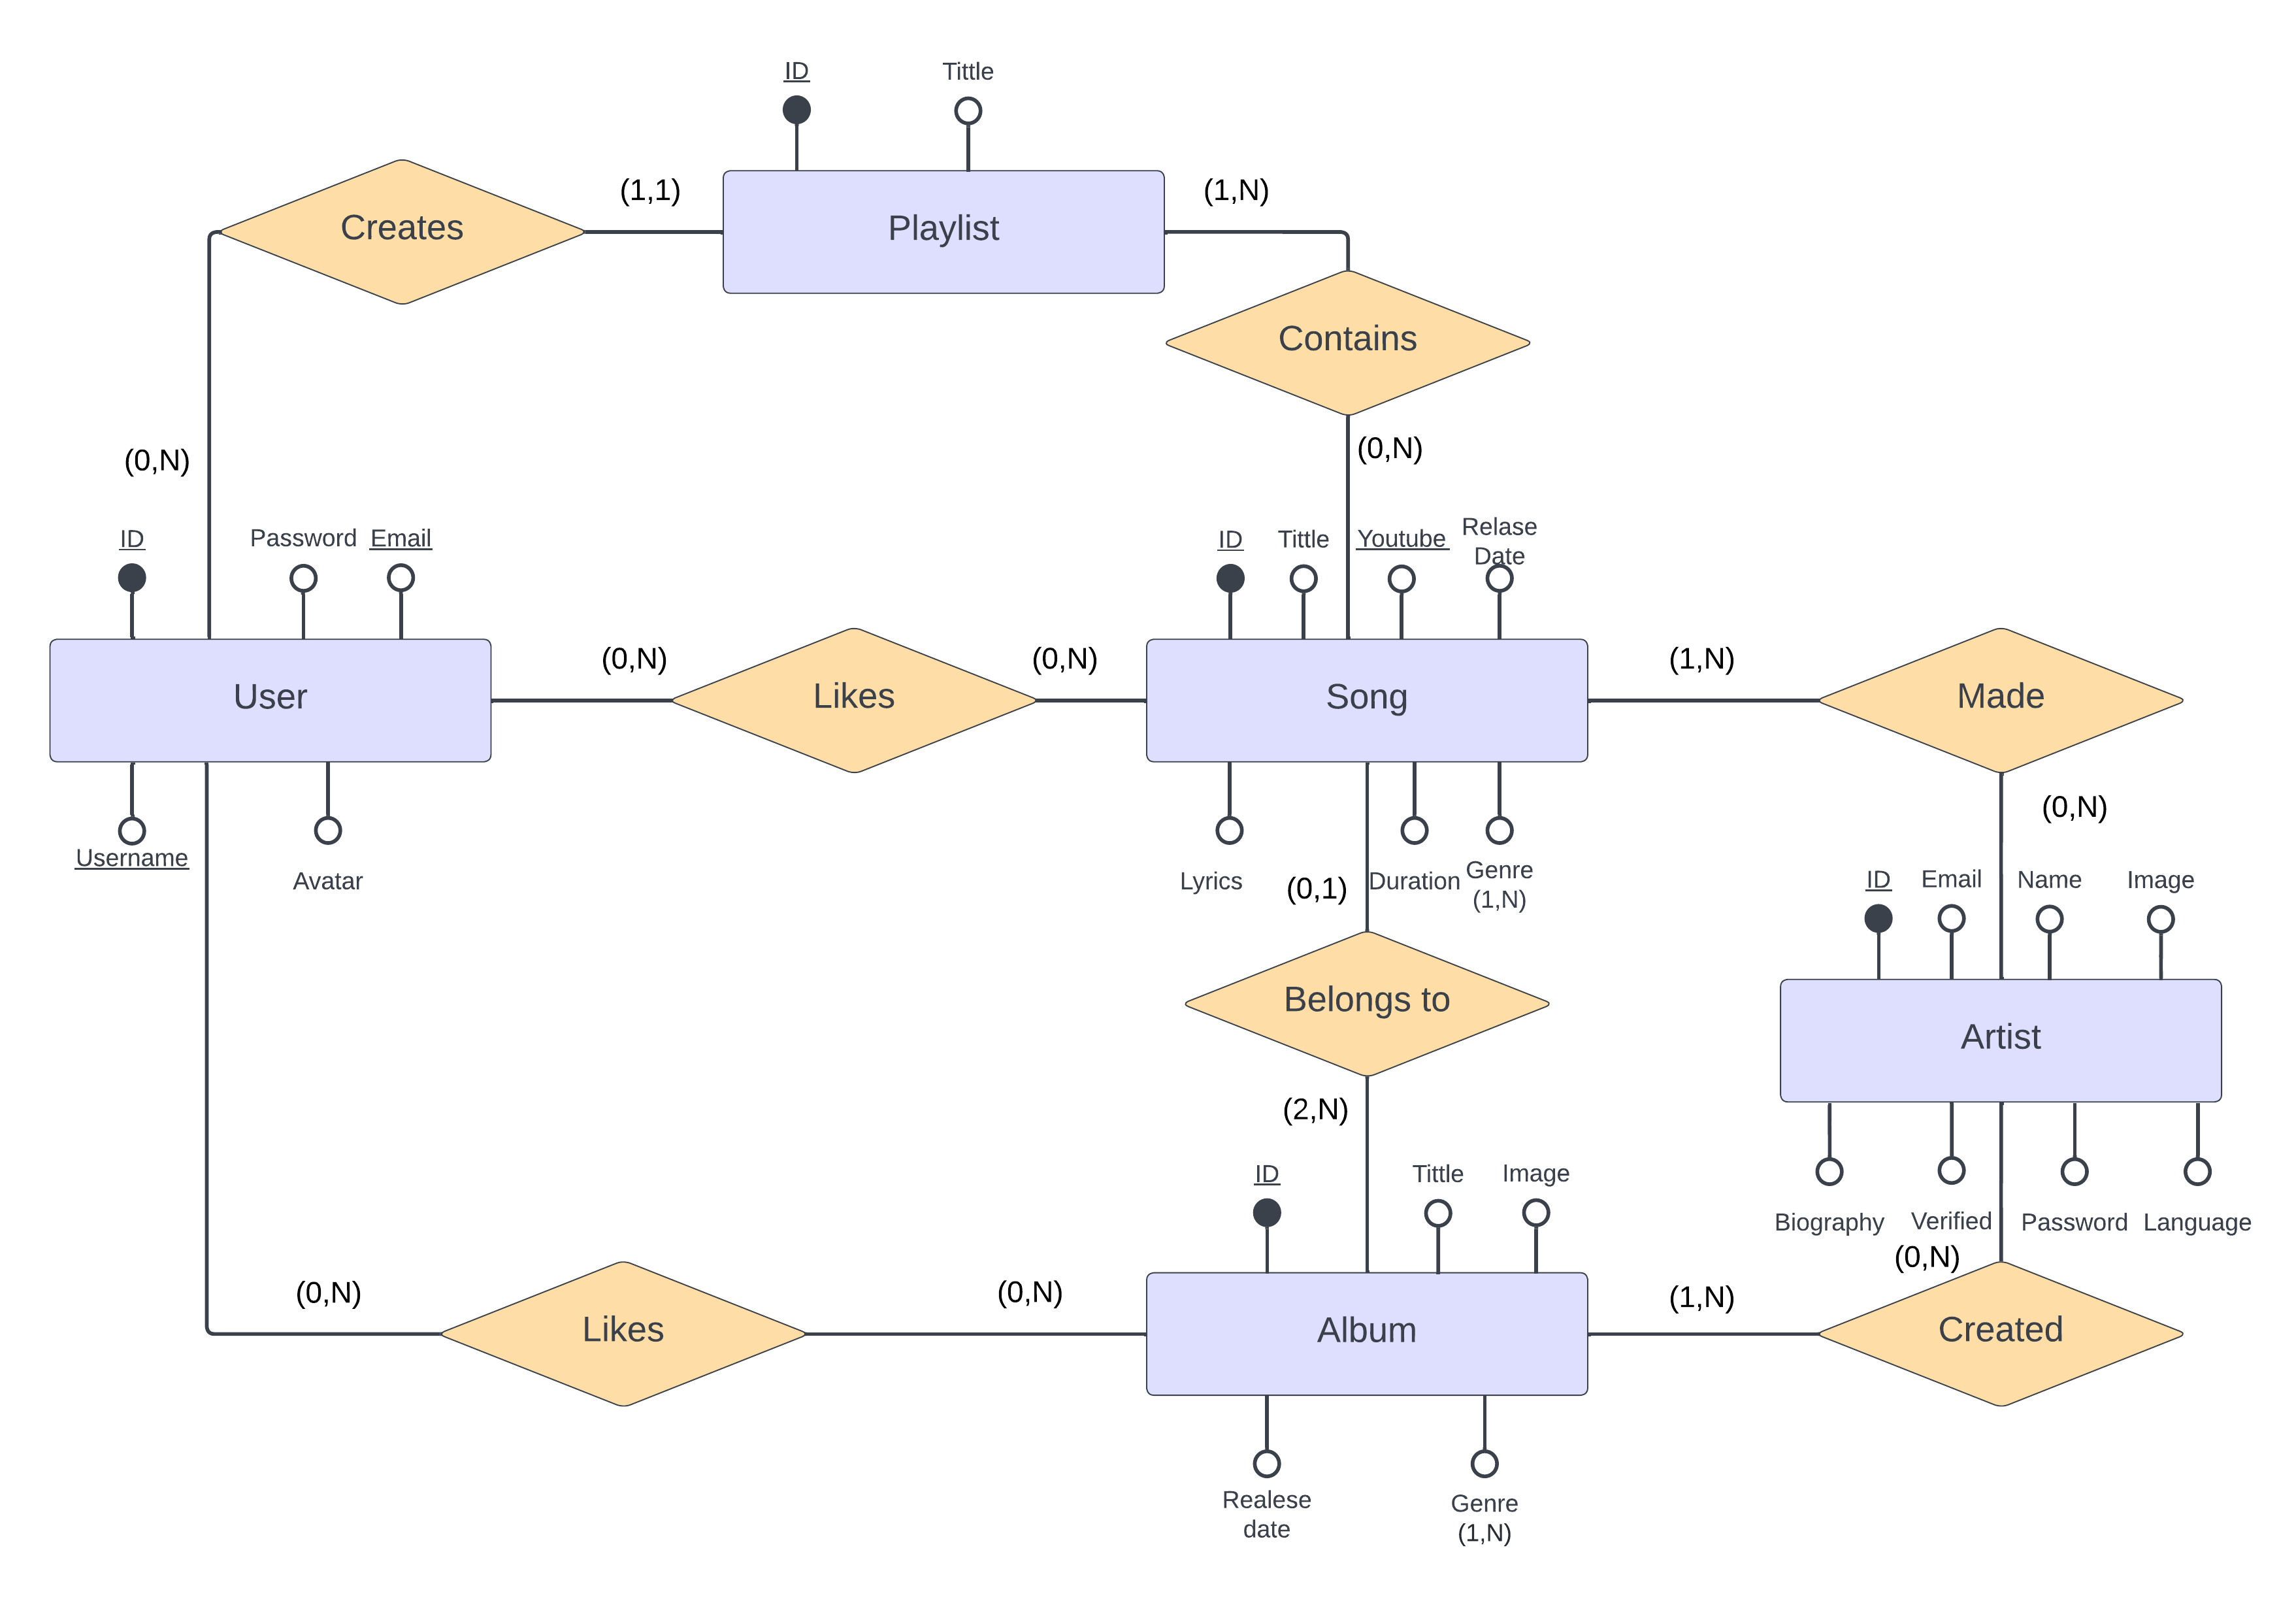
\includegraphics[width=0.9\textwidth]{sections/DLL/BD_ER_SCHEMA.png}
\caption{ER Schema diagram}
\end{figure}

%Describe here your ER schema


The ER schema contains the following entities:
\begin{itemize}
    \item \textbf{Users}: describes the user that will use our web application. Each user has as a primary key a serial ID that is given the moment the account is created. For each user we also record the email, their password, which can have length between 8 and 24 characters, and their username and an avatar image provided from a list of possible options.

    \item \textbf{Songs}: each song is uniquely determined by a serial ID number, given the moment the song is uploaded. It also contains some data of the song, such as the tittle, YouTube link to the music video, release date, the duration of the song, list of genres the song belongs to and the lyrics of the song.

    \item \textbf{Playlist}: is a list of songs that a user creates. As a primary key it has an ID and as attribute a tittle. Also, as a foreign key we have the User ID, which refers to the owner and creator of the playlist.

    \item \textbf{Artist}: similar to an user but need a verification in order to create the account. As identifier it has a serial ID number and has a name, an image, a biography, a verification boolean in order to upload songs and a language in which most of its songs are written. Also an artist has an email and a password, which can have a length between 8 and 24 characters

    \item \textbf{Album}: is a collection of songs that are created by an artist. They are recognized by a serial ID and also have a tittle, a image that is the cover of the album, a release date and a list of genres it belongs to.
\end{itemize}

Now we dive into the relationships between our entities:

\begin{itemize}
    \item \textbf{Creates}: an user can create a playlist, which is only owned and created by one user, this is that there are not collaborative playlist. An user can have none playlist or as much as he wishes. In summary, is a 1-N relationship.
    \item \textbf{Contains}: is the relation between playlist and song, in which is described that a playlist must have at least one song and no maximum amount; and a song can be or not be in a playlist. It is a N-N relationship. In the SQL database is represented by the name "SongsInPlaylists".
    \item \textbf{Likes}: an user has the ability to like songs. A new user will begin without any liked songs and as the user likes more songs, the list will grow. A song can either be liked or not by an user. In the SQL database is represented by the name "LikedSongs".
    \item \textbf{Likes}: an album can be liked by many different users, and a user can like or not any album, new users will not like any album until they like the first one. In the SQL database is represented by the name "LikedAlbums".
    \item \textbf{Belongs to}: A song can belong to one album or be a single, which means that it does not belong to any album. Albums must at least have two songs, in case of one song only, it would be consider to be a single song and not an album itself. In the SQL database is represented by the name "SongsInAlbums".
    \item \textbf{Made}: is the relationship between songs and artists. An artist can make no songs (can not upload songs until the verification is completed) or have plenty of them. A song must be created for at least one artist, and in case of a collaboration, more than one artist.
    \item \textbf{Created}: Albums are created by at least one artist, and must be uploaded by the artist itself. An artist can have no albums (just upload single songs) at all or to have one or more albums.
\end{itemize}




\begin{figure}[h]
\centering
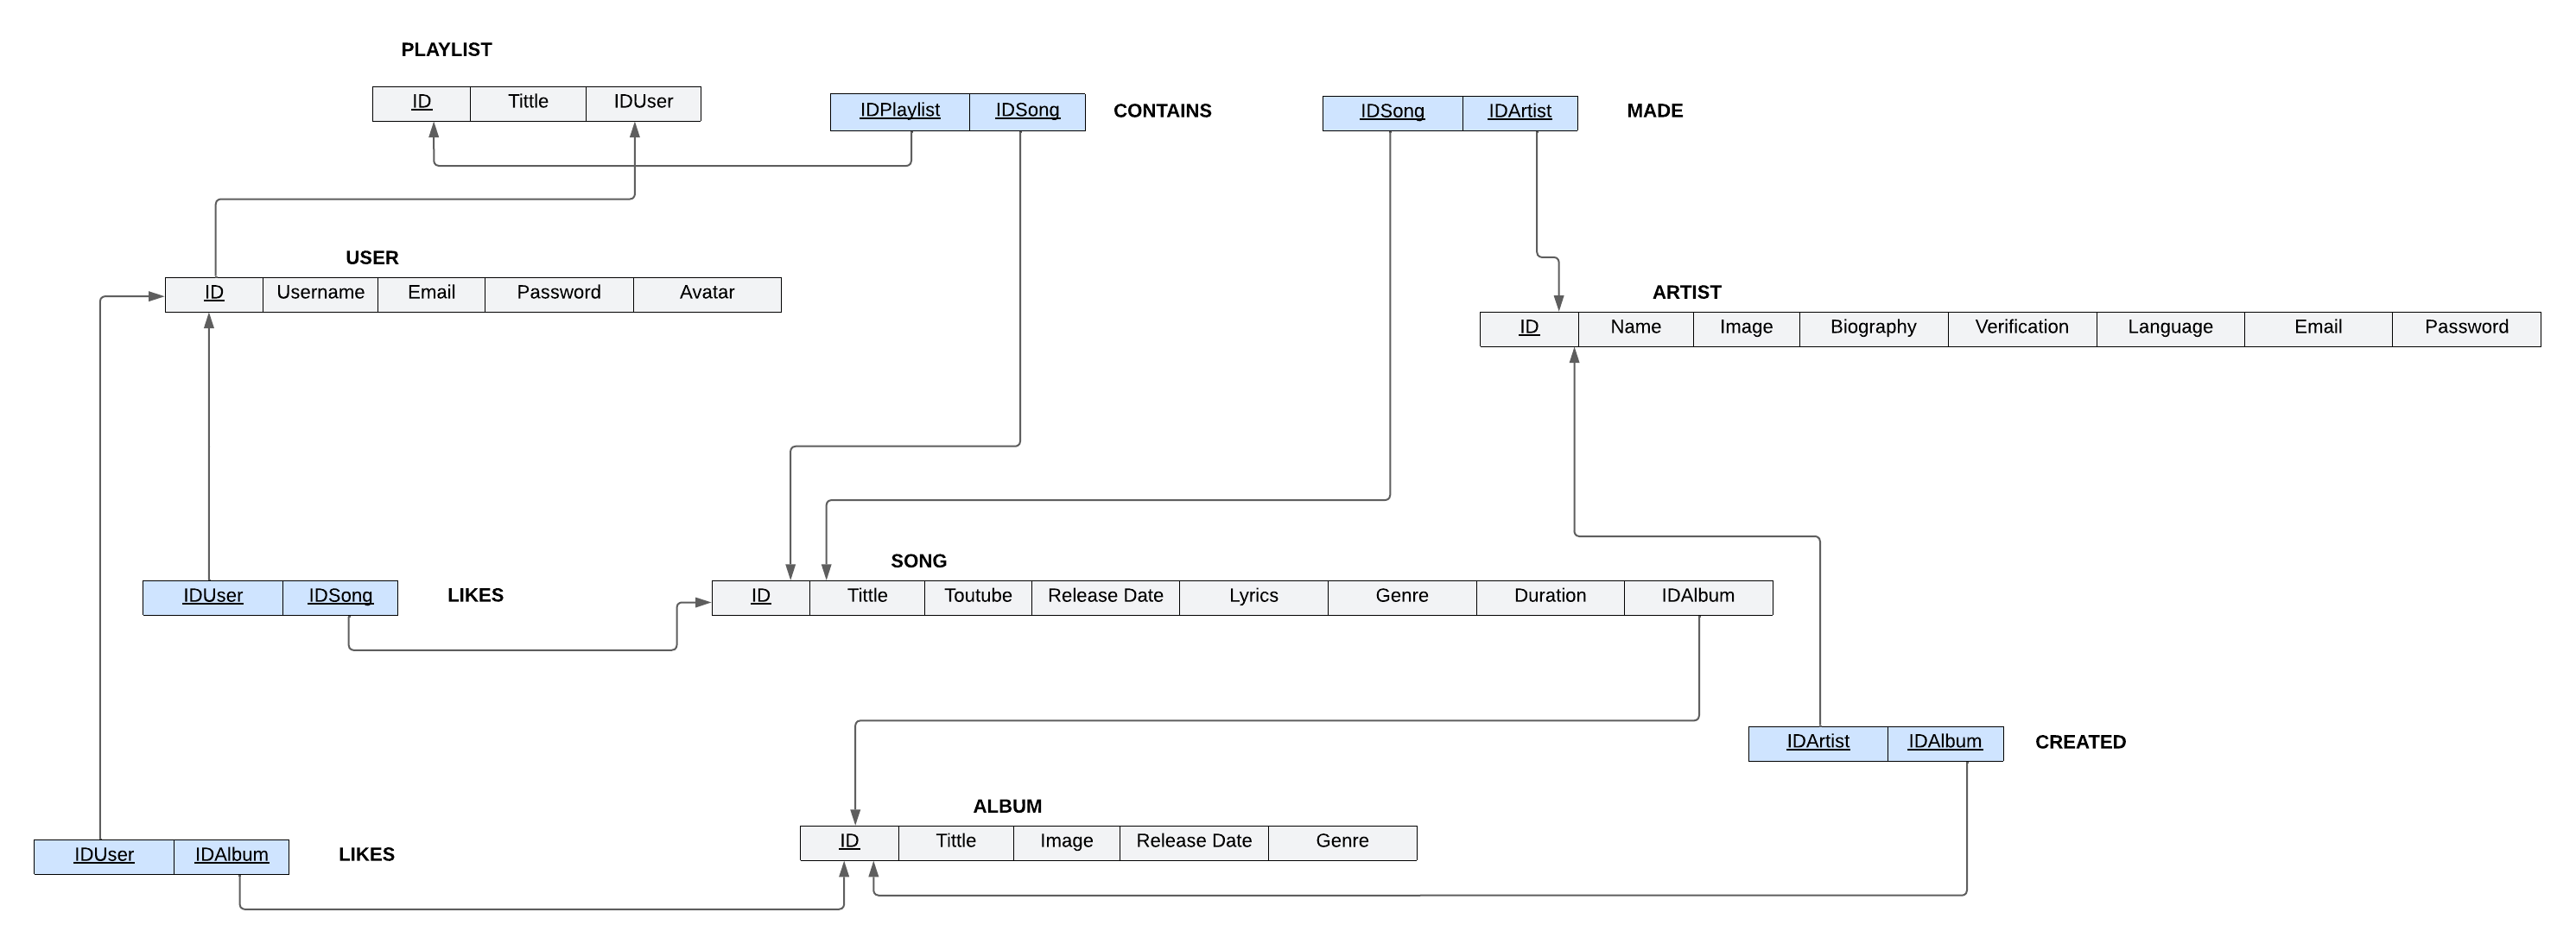
\includegraphics[width=1.1\textwidth]{sections/DLL/BD_ER_TABLE.png}
\caption{ER Tables Diagram}
\end{figure}




